\chapter{Fundamentação Teórica}

	% Neste capítulo será apresentado os conceitos de rastreamento, localização e identificação nos quais o trabalho se fundamenta. A partir dessa teoria será possível entender melhor a proposta do projeto.

	Em ambientes inteligentes, as informações de contexto sobre os usuários presentes como localização e identidade são de grande importância proporcionando uma maior acurácia nas tomadas de decisões. Informações de contexto como essas são muito complicadas de obter devido a dinamicidade do ambiente, no qual usuários entram e saem a todo momento e interagem com diversos equipamentos.

	Para obter essas informações é necessário utilizar técnicas de identificação e localização mescladas com técnicas de rastreamento.

	O rastreamento pode ser definido como o problema de estimar a trajetória de uma entidade em um plano de imagem a medida em que se move na cena. Em outras palavras, um rastreador atribui rótulos as entidades monitoradas em diferentes quadros de um vídeo~\cite{yilmaz}.

	Em um ambiente inteligente, o rastreamento de pessoas é uma das principais ferramentas para detectar novos usuários e serve como base para que novas informações possam ser colhidas. Por exemplo, para que seja possível realizar reconhecimento facial de uma pessoa é necessário, primeiramente, obter imagens de sua face, porém isso só é possível se soubermos onde tal pessoa se encontra na imagem, ou seja, é necessário detectá-la e rastreá-la.

	Com o rastreamento mesclado com informações de profundidade é possível, também, obter a localização física das pessoas rastreadas. Tal informação é muito útil em um ambiente inteligente pois, a posição do usuário, possibilita maiores possibilidades para as tomadas de decisões.

	Neste capítulo é mostrada uma abordagem conceitual sobre rastreamento de entidades, localização e identificação das mesmas em um ambiente. 

	Sobre rastreamento é mostrada uma visão geral do processo e quais as dificuldades mais comuns encontradas, bem como as técnicas mais comuns de detecção e rastreamento, as diferentes maneiras de representar as entidades rastreadas e algumas de suas características utilizadas. 

	Sobre localização é mostrada uma visão geral de como obter a posição relativa a uma câmera utilizando imagens de profundidade.

	Sobre identificação é mostrado conceitos gerais sobre biometria e as características biométricas existentes. Sobre reconhecimento facial, é apresentado os conceitos gerais e conceitos mais específicos das diferentes etapas do processo de reconhecimento: detecção de faces e reconhecimento das mesmas. Além desses conceitos, é apresentado alguns métodos utilizados atualmente em cada uma dessas etapas.





% \section{Rastreamento e Localização}

	% O rastreamento de entidades, como pessoas ou objetos, é uma importante tarefa
	% do campo da computação visual. A proliferação de computadores com um alto poder
	% computacional, a disponibilidade de câmeras de alta qualidade a um preço
	% acessível e a crescente necessidade de sistemas automáticos de análise de
	% vídeos têm gerado um grande interesse em algoritmos de rastreamento~\cite{yilmaz}.

	% Em um ambiente inteligente, o rastreamento de pessoas é uma das principais
	% ferramentas para detectar novos usuários e serve como base para que novas
	% informações possam ser colhidas. Por exemplo, para que seja possível realizar
	% reconhecimento facial de uma pessoa é necessário, primeiramente, obter imagens
	% de sua face, porém isso só é possível se soubermos onde tal pessoa se encontra
	% na imagem, ou seja, é necessário detectá-la e rastreá-la.

	% Com o rastreamento mesclado com informações de profundidade é possível,
	% também, obter a localização física das pessoas rastreadas. Tal informação é
	% muito útil em um ambiente inteligente pois, a posição do usuário,
	% possibilita maiores possibilidades para as tomadas de decisões.

	% Neste capítulo será mostrada uma abordagem conceitual sobre rastreamento de
	% entidades e localização das mesmas em um ambiente. Sobre rastreamento será
	% mostrada uma visão geral do processo e quais as dificuldades mais comuns
	% encontradas, bem como as técnicas mais comuns de detecção e rastreamento, as
	% diferentes maneiras de representar as entidades rastreadas e algumas de suas
	% características utilizadas. Sobre localização será mostrada uma visão geral de
	% como obter a posição relativa a uma câmera utilizando imagens de profundidade.

	\section {Rastreamento}	

	Rastreamento de objetos é uma importante tarefa do campo da computação visual. A proliferação de computadores com um alto poder computacional, a disponibilidade de câmeras de alta qualidade e preço acessível e a crescente necessidade de sistemas automáticos de análise de vídeos têm gerado um grande interesse em algoritmos de rastreamento de objetos~\cite{yilmaz}.

	Basicamente, rastreamento pode ser definido como o problema de estimar a trajetória de um objeto em um plano de imagem a medida em que se move na cena. Em outras palavras, um rastreador atribui \textit{labels} para os objetos monitorados em diferentes quadros de um vídeo~\cite{yilmaz}.

	A detecção e o rastreamento de pessoas tem um grande potencial em aplicações em domínios tão diversos como animação, interação humano-computador, vigilância automatizada (monitorar uma cena para detectar atividades suspeitas), entre outros. Por esta razão, tem havido um crescimento notável na investigação deste problema.

	O rastreamento de pessoas em um ambiente é considerada como uma tarefa complexa devido a:

		\begin{enumerate}
			\item complexidade do corpo humano;
			\item alta dinamicidade do ambiente;
			\item ruído nas imagens~\cite{yilmaz};
			\item complexidade do movimento das pessoas;
			\item oclusões parciais ou totais de pessoas;
			\item variação na iluminação do ambiente~\cite{yilmaz};
			\item processamento em tempo-real~\cite{yilmaz};
		\end{enumerate}

	Algumas dessas dificuldades podem ser vencidas com a utilização de imagens de profundidade ao invés de imagens de cor ou intensidade. As imagens de profundidade, além de serem muito pouco sensíveis as variações de iluminação, provê um fácil entendimento da estrutura da cena, que pode ser utilizada para simplificar as tarefas de rastreamento. Além disso, as câmeras que provêm imagens de profundidade estão comercialmente disponíveis a um preço acessível~\cite{nikos}.

	Várias abordagens para rastreamento de objetos já foram propostas. Basicamente, elas se diferem na forma que tratam as seguintes perguntas~\cite{yilmaz}: 
		
		\begin{itemize}
			\item Qual representação do objeto é adequada para o rastreamento?
			\item Quais características na imagem devem ser utilizadas?
			\item Como o movimento, aparência e a forma do objeto deve ser modelada? 
		\end{itemize}

	As respostas para estas perguntas dependem do contexto/ambiente onde o rastreamento será utilizado e do uso final das informações de rastreamento~\cite{yilmaz}.

	O rastreamento de pessoas geralmente inicia com o processo de segmentação da imagem da pessoa do resto da imagem. Depois, essas imagens segmentadas são transformadas em outras representações para reduzir a quantidade de informação ou para atender a um determinado algoritmo. Com isso, deve-se definir como as pessoas vão ser rastreadas \textit{frame} a \textit{frame}~\cite{moeslund}.

	Basicamente, o processo de rastreamento pode ser dividido em duas etapas:

		\begin{enumerate}
			\item Detecção do objeto;
			\item Rastreamento do objeto detectado;
		\end{enumerate}

	Antes de falarmos mais sobre cada uma dessas etapas e os métodos existentes para cada, vamos falar sobre as maneiras existentes de representar os objetos rastreados e sobre as características nas imagens que podem ser utilizadas.

%%%%%%%%%%%%%%%%%%%%%%%%%%%%%%%%%%%%%%%%%%%%%%%%%%%%%%%%%%%%%%%%%%%%%%%%%%%%%%%%%%%%%%%%%%%%%%%%%%%%%%%%%%%%%%%

\subsection{Representação do Objeto}

	Nos sistemas de rastreamento, os objetos rastreados devem ser representados de alguma maneira. Geralmente, as representações são baseados em suas formas. Existe uma forte relação entre a representação do objeto e o algoritmo de rastreamento escolhido~\cite{yilmaz}. A representação é escolhida baseada no domínio da aplicação e as mais utilizadas são:

	\begin{figure}[hbt]
		\begin{center}
			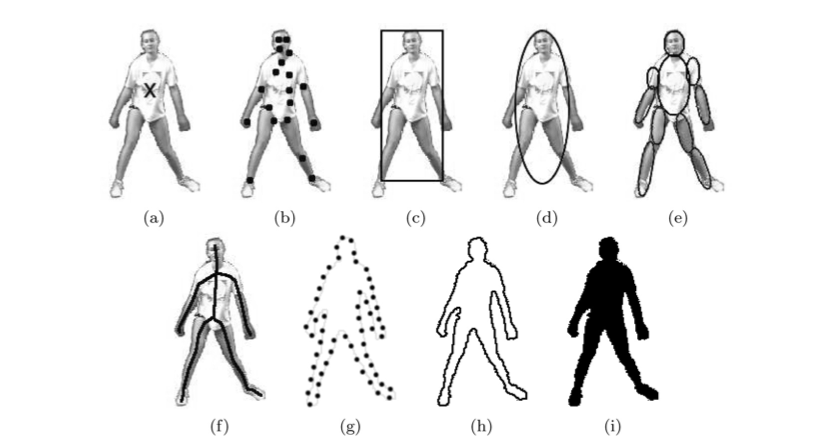
\includegraphics[scale=0.5]{figuras/2.FundamentacaoTeorica/representacao.png}
		\end{center}
		\caption{Representações de objetos rastreados. (a) Centroide, (b) múltiplos pontos, (c) representação retangular, (d) representação elíptica, (e) representação de múltiplas partes, (f) esqueleto do objeto, (g) contorno do objeto por pontos,(h) contorno completo do objeto, (i) silhueta do objeto~\cite{yilmaz}}
		\label{representacao}
	\end{figure}

	\begin{itemize}
		\item \textbf{Pontos:} o objeto é representado por um ponto, como por exemplo a centroide~\cite{veenman} da Figura \ref{representacao}(a), ou por vários pontos~\cite{serby}, como por exemplo na Figura \ref{representacao}(b). Essa representação é mais adequada para rastreamento de objetos que ocupam uma pequena região na imagem~\cite{yilmaz};

		\item \textbf{Formas geométricas primitivas:} o objeto é representado por formas geométricas simples como um retângulo ou uma elipse, como mostrados nas Figuras \ref{representacao}(c) e (d)~\cite{comaniciu}. Essa representação é mais adequada para simples objetos rígidos~\cite{yilmaz};

		\item \textbf{Silhueta e Contorno:} representação por contorno define os limites de um objeto, como mostrado nas Figuras \ref{representacao}(g) e (h). A região interna do contorno é chamada de Silhueta, como mostrado na Figura \ref{representacao}(i). Essa representação é mais adequada para rastrear objetos complexos de forma não rígida~\cite{yilmaz, yilmaz2}. Ela é popular devido a sua simplicidade. A silhueta ou contorno de um objeto pode ser obtida definindo métodos de limiarização ou subtração, podendo ser utilizada tanto com imagens 2D quanto 3D. A representação 2D geralmente é mais simples~\cite{moeslund};

		\item \textbf{Modelos de formas articuladas:} objetos articulados são compostos por partes do corpo que se ligam por meio de juntas. Para representar objetos articulados, utiliza-se figuras geométricas para cada parte do corpo, como mostrado na Figura \ref{representacao}(e)~\cite{yilmaz};

		\item \textbf{Modelos de esqueletos:} modelos de esqueletos são extraídos do objeto rastreado, como mostrado na Figura \ref{representacao}(f). Essa representação pode ser utilizada tanto para objetos articulados rígidos quanto não rígidos~\cite{yilmaz};
	\end{itemize}

	Para rastreamento de pessoas a representação por meio de contorno ou silhuetas são as mais adequadas~\cite{yilmaz}.

	O rastreamento de várias pessoas de maneira simultânea é considerada uma tarefa muito complexa. As representações das pessoas rastreadas podem se dividir ou fundir em novas representações devido a possíveis oclusões ou ruídos na imagem, e a aparência do objeto pode variar devido a sombras e mudanças da iluminação~\cite{moeslund}.

%%%%%%%%%%%%%%%%%%%%%%%%%%%%%%%%%%%%%%%%%%%%%%%%%%%%%%%%%%%%%%%%%%%%%%%%%%%%%%%%%%%%%%%%%%%%%%%%%%%%%%%%%%%%%%%

\subsection{Características para rastreamento}

	A seleção das características é uma tarefa crítica para o rastreamento e está fortemente relacionada com a representação do objeto. Em geral, a seleção procura as características mais singulares para que o objeto rastreado seja facilmente distinguido~\cite{yilmaz}. As características mais comuns utilizadas atualmente são:

	\begin{itemize}
		\item \textbf{Cor:} a cor do objeto é influenciada principalmente por duas características: a distribuição da iluminação e a propriedade de reflectância do objeto. Geralmente, a representação \textit{RGB} é utilizada para representar a cor~\cite{yilmaz};

		\item \textbf{Borda:} os limites de um objeto geram uma grande variação na intensidade na imagem e são menos sensíveis a variações na iluminação comparado com as cores. A detecção por meio das bordas é utilizada para identificar essas variações de intensidade na imagem. Os algoritmos que detectam as bordas do objeto geralmente as utilizam para representação dos mesmos~\cite{yilmaz};

		\item \textbf{Fluxo óptico:} é um campo denso de vetores de deslocamento que define a tradução de cada \textit{pixel} em uma região. Ele é calculado a partir da restrição de luminosidade, que pressupõe a constância de brilho de \textit{pixels} correspondentes nas \textit{frames} consecutivas~\cite{yilmaz, horn};

		\item \textbf{Textura:} é a medida da intensidade da variação da superfície que quantifica propriedades como suavidade e regularidade. A Textura é menos sensível a variação da iluminação comparado com a cor~\cite{yilmaz};

	\end{itemize}

De todas as características, a mais utilizada para rastreamento é a cor~\cite{yilmaz}.

%%%%%%%%%%%%%%%%%%%%%%%%%%%%%%%%%%%%%%%%%%%%%%%%%%%%%%%%%%%%%%%%%%%%%%%%%%%%%%%%%%%%%%%%%%%%%%%%%%%%%%%%%%%%%%%

\subsection{Detecção de objeto}

	Todo método de rastreamento requer um mecanismo de detecção de objetos que pode ser realizada a cada \textit{frame} obtida ou na primeira vez que o objeto aparece no vídeo. Os método mais populares são:


	\begin{itemize}
		\item \textbf{Detector de pontos:} esses detectores são usados para encontrar pontos de interesses dentro da imagem que tem uma expressiva textura na sua respectiva localização. Pontos de interesse são amplamente usados no contexto do movimento e no rastreamento. A qualidade desejável para o ponto de interesse é que seja invariante diante das mudanças de iluminação e ângulo de visão da câmera~\cite{yilmaz}.
	
		\item \textbf{Subtração de fundo:} é um método popular para segmentação de movimento, especialmente nas situações em que o plano de fundo é relativamente estático. Ele detecta as regiões de movimento na imagem obtendo a diferença \textit{pixel} a \textit{pixel} entre a \textit{frame} corrente e a \textit{frame} referente ao plano de fundo~\cite{weiming}. Geralmente, um algoritmo de componentes conectadas é aplicado para obter regiões conectadas que correspondem a um objeto~\cite{yilmaz}.

		\item \textbf{Segmentação:} o objetivo do algoritmo de segmentação é particionar a imagem em regiões com certo grau de similaridade. Todo algoritmo de segmentação tem dois problemas: o critério para definir uma boa partição e o método para arquivar particionamentos eficientes~\cite{yilmaz, shi}.

		\item \textbf{Aprendizagem supervisionada:} a detecção de objetos pode ser feita pelo aprendizado automático de diferentes objetos de um conjunto de exemplos por meio de um mecanismo de aprendizado. Esse aprendizado requer o armazenamento de um um conjunto de \textit{templates}. A partir desse conjunto de informações, o algoritmo gera uma função que mapeia as possíveis entradas para as saídas desejadas. Um problema padrão é a classificação onde a função gera um valor contínuo a partir de um determinado comportamento do objeto. No contexto da detecção de objetos as informações armazenadas são compostas por um par de características de objetos e uma classe associada onde ambos os valores são manualmente definidos. Seleção de características tem um papel importante no desempenho da classificação, portanto, é importante usar um conjunto de características que seja possível discriminar uma classe das outras~\cite{yilmaz}.
	\end{itemize}

%%%%%%%%%%%%%%%%%%%%%%%%%%%%%%%%%%%%%%%%%%%%%%%%%%%%%%%%%%%%%%%%%%%%%%%%%%%%%%%%%%%%%%%%%%%%%%%%%%%%%%%%%%%%%%%

\subsection{Rastreamento de objeto}

	O objetivo do rastreamento de objetos é conhecer a trajetória do mesmo no tempo localizando sua posição em cada \textit{frame}. O rastreamento de objetos também pode prover a região completa na imagem ocupada pelo objeto a cada instante~\cite{yilmaz}. 

	As atividades de detecção de objetos e de estabelecimento de correspondências entre os objetos e as instâncias dos \textit{frames} podem ser realizadas tanto separadamente como concomitantemente. No primeiro caso, as prováveis regiões de objetos são obtidas e o rastreador encontra correspondência entre os objetos e os \textit{frames}. No último caso, as prováveis regiões e as correspondências são feitas juntas e estimadas pela atualização iterativa da localização do objeto e de regiões de informações obtidos dos \textit{frames} anteriores~\cite{yilmaz}.

	Os métodos de rastreamento de objetos mais utilizados atualmente são:

	\begin{itemize}
		\item \textbf{Rastreamento de pontos:} os objetos detectados a cada frame são representados por pontos e a associação entre os pontos é feita com base no estados anterior do objeto que pode incluir a posição e o movimento. Essa abordagem requer um mecanismo externo para detectar o objeto a cada \textit{frame}~\cite{yilmaz};

		\item \textbf{Rastreamento de \textit{kernel}}: os objetos são rastreados pelo cálculo do movimento do \textit{kernel} em \textit{frames} consecutivas. Esse movimento geralmente esta na forma de transformações paramétricas como translação e rotação. \textit{Kernel} se refere ao formato ou aparência do objeto~\cite{yilmaz}.

		\item \textbf{Rastreamento de silhuetas:} o rastreamento é feito estimando a região do objeto a cada \textit{frame}. Esse método utiliza informação contida dentro da região do objeto. Esta informação pode ser na forma de densidade de aparência e modelos de forma que estão, geralmente, na forma de mapas de borda. Dado os modelos de objeto, silhuetas são rastreadas por qualquer forma de correspondência ou evolução de contorno. Ambos os métodos podem ser essencialmente considerados como segmentação de objetos aplicada no domínio temporal utilizando os priores gerados a partir dos \textit{frames} anteriores~\cite{yilmaz}.
	\end{itemize}

	Com os objetos rastreados, para obtermos a posição dos mesmos devemos obter informações de profunidade. Na próxima seção falaremos sobre como essas informações são obtidas utilizando imagens de profunidade.





	\section{Localização}
\label{sec:luz-estruturada}

	Calcular a distância de vários pontos na cena relativa a posição da câmera é uma
	importante tarefa de sistemas de computação visual~\cite{jain}. Para isso,
	deve-se obter informações de profundidade das entidades em interesse. Essas
	informações podem ser obtidas utilizando imagens de intensidade ou de
	profundidade.
	
	Uma maneira comum de se obter informações de profundidade de imagens de
	intensidade é adquirir um par de imagens usando duas câmeras deslocadas entre si
	por uma distância conhecida. Como alternativa, duas ou mais imagens obtidas de
	uma câmera em movimento também pode ser utilizadas para calcular informações de
	profundidade~\cite{jain}. Esse método é conhecido como \textit{Stereo Vision} e
	necessita ser bem calibrado.  Além disso, os algoritmos que o implementa
	geralmente são computacionalmente caros e não funcionam em ambiente com baixa
	condição de iluminação~\cite{fall-detection}.
	
	Informações de profundidade também podem ser obtidas indiretamente através de
	imagens de intensidade utilizando sinais na imagem, como sombreamento e
	textura~\cite{jain}.
	
	Em contraste com imagens de intensidade, imagens cujo valor em cada pixel é uma
	função da distância do ponto correspondente na cena do sensor são chamadas de
	imagens de profundidade, exemplificada na Figura \ref{depthimage}. Tais imagens
	podem ser adquiras diretamente utilizando sensores específicos~\cite{jain}.
	Alguns dos métodos mais conhecidos são:

	\begin{figure}[htb]
		\begin{center}
			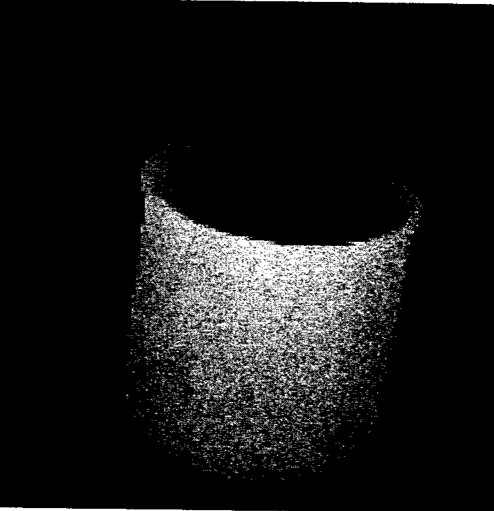
\includegraphics[scale=0.3]{figuras/2.FundamentacaoTeorica/depthimage.png}
		\end{center}
		\caption{Imagem de profundidade de uma caneca de café~\cite{jain}.}
		\label{depthimage}
	\end{figure}

	\begin{enumerate}
		\item \textbf{Triangulação:} utiliza as propriedades geométricas do triângulo
		para calcular a localização de entidades. Pode ser dividida em duas
		subcategorias: lateração e angulação. Lateração computa a posição de uma
		entidade estimando sua distância de múltiplos ponto de referência. Calcular a
		posição de uma entidade em duas dimensões requer estimativas de distância de
		três pontos não colineares como mostrado na Figura \ref{fig:lateration}. Já em
		três dimensões são necessários quatro pontos não coplanares. Ângulação utiliza
		ângulos para determinar a distância da entidade. Em geral, ângulação em duas
		dimensões requer estimativas de dois ângulos e a estimativa da distância entre
		dois pontos de referência como mostrado na Figura
		\ref{fig:angulation}~\cite{triangulacao};
		
		\begin{figure}[htb]
			\begin{center}
				\subfloat[Lateração] {
					\label{fig:lateration}
					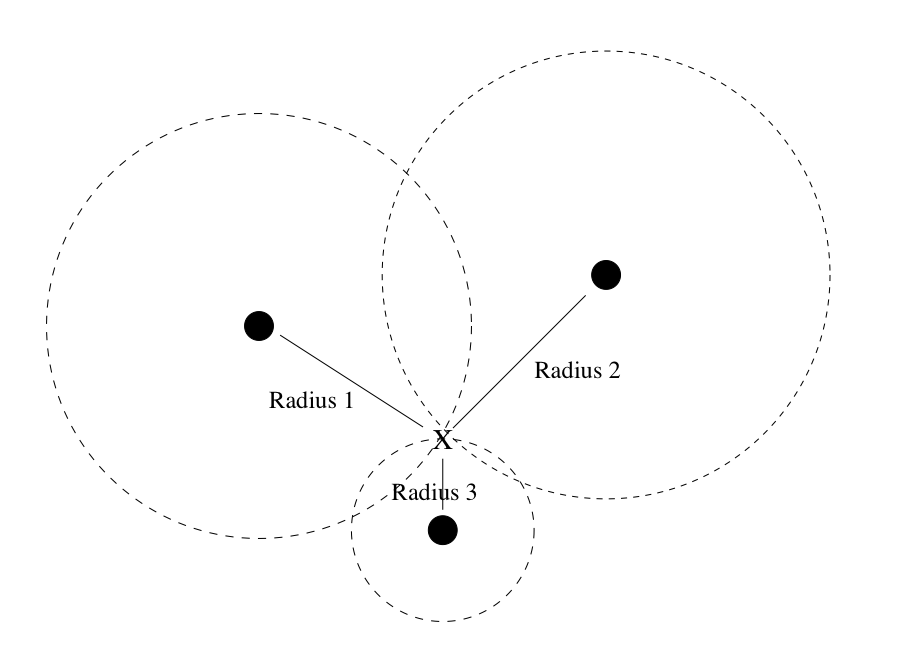
\includegraphics[width=0.45\textwidth]{figuras/2.FundamentacaoTeorica/lateration.png}}
				\subfloat[Angulação] {
					\label{fig:angulation}
					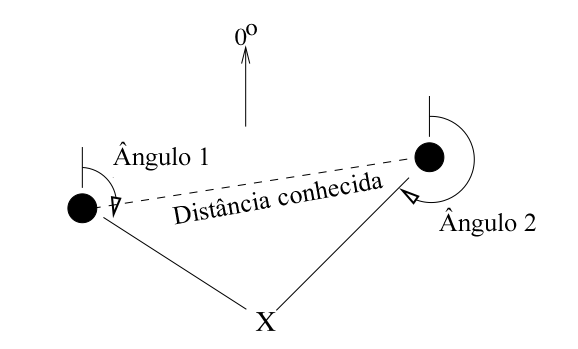
\includegraphics[width=0.45\textwidth]{figuras/2.FundamentacaoTeorica/angulation.png}}
			\end{center}
			\caption{ (a) Determina a distância em duas dimensões utilizando lateração.
			Requer a distância entre a entidade $\displaystyle X$ e três pontos de referência não colineares~\cite{triangulacao}.}
			(b) Exemplo de uma angulação em duas dimensões em que se localiza a
			entidade $\displaystyle X$ utilizando ângulos relativos a um vetor de
			referência $\displaystyle 0º$ e a distância entre dois pontos de referência~\cite{triangulacao}.}
		\end{figure}

		\item \textbf{Tempo de Vôo (TOF - \textit{Time of flight}):} a distância até a
		entidade é calculada observando a diferença de tempo entre o pulso
		eletromagnético transmitido e recebido. A informação de profundidade também pode
		ser obtida através da detecção da diferença de fase entre as ondas transmitidas
		e as recebidas de um feixe de amplitude modulada~\cite{jain, fall-detection}.
		Câmeras TOF provêem imagens de profundidade com melhor acurácia em relação ao
		método de \textit{Stero Vision}, porém são muito caras e pouco
		acessíveis~\cite{fall-detection};
		
		\item \textbf{Luz Estruturada:} uma imagem de
		profundidade não pode ser obtida utilizando somente um sensor de vídeo. Porém,
		adicionando uma textura artificial na cena, como na
		Figura~\ref{fig:structured-light}, uma imagem de profundidade pode ser
		recuperada. Esse princípio consiste na projeção de pontos de luz infra-vermelhos
		na cena que são recuperados por uma câmera infra-vermelha que lê a textura.
		Trata-se de um método mais acessível que o TOF, porém é pouco eficiente
		para estimar a distância dos pontos nas bordas dos objetos e em áreas muito
		longe do sensor~\cite{fall-detection};
		
		\begin{figure}[htb]
			\begin{center}
				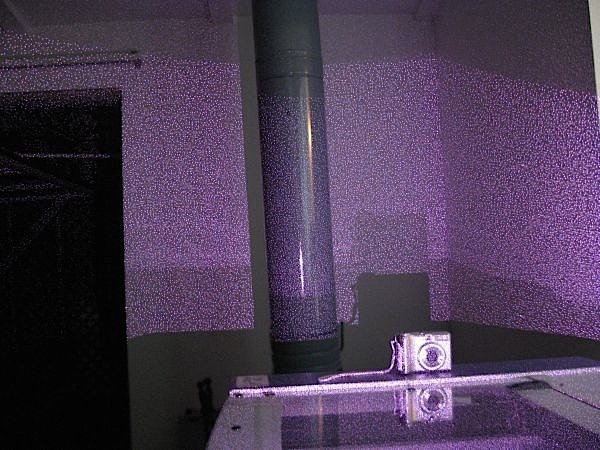
\includegraphics[width=0.45\textwidth]{figuras/2.FundamentacaoTeorica/structured-light.jpg}
			\end{center}
			\caption{Exemplo de uma textura artificial adicionada a cena por meio de
			pontos de luz infra-vermelha utilizando o método Luz Estruturada~\cite{img-strutuctured-light}.}
			\label{fig:structured-light}
		\end{figure}
	\end{enumerate}

	Imagens de profundidade são úteis devido a sua especificação explícita de
	valores de profundidade. Ao mesmo tempo acreditava-se que se a informação de
	profundidade fosse disponibilizada de maneira explícita, o processamento
	posterior da imagem seria facilitado. Tornou-se claro que a informação de
	profundidade ajuda, porém a tarefa básica de interpretação de imagens mantém
	todas as suas dificuldades~\cite{jain}.



	

\section{Identificação}
	
	Um ambiente ubíquo capaz de identificar seus usuários, pode prover uma
	personalização automática do ambiente de acordo com as preferências do usuário e
	até mesmo prover um ambiente mais seguro com controle de acesso físico e
	prevenção de fraudes \cite{saocarlos}. A identificação de um usuário em um
	ambiente inteligente é feita por meio de sistemas de reconhecimento automático.
	Há alguns anos, um grande número de pesquisas vem sendo desenvolvidas para criação
	deste tipo de sistema  \cite{saocarlos}.
	
	As abordagens de identificação pessoal que utilizam ``alguma coisa que você
	sabe'', como um número de identificação pessoal (PIN - \textit{Personal
	Identification Number}), ou ``alguma coisa que você tenha'', como um cartão de identificação,
	não são confiáveis o suficiente para satisfazer os requisitos de segurança de um
	sistema de identificação porque não têm a capacidade de diferenciar um usuário
	legítimo de um impostor que adquiriu de forma ilegal o privilégio de acesso
	\cite{hong}. Esta fragilidade pode ser evitada utilizando biometria: alguns
	traços físicos ou comportamentais são muito mais complicados de serem forjados
	que uma cadeia de caracteres \cite{drovetto}.
	
	Hoje em dia, várias técnicas de reconhecimento biométrico por meio de faces,
	íris, voz, entre outras, vêm sendo estudadas e utilizadas em sistemas de
	reconhecimento automático \cite{bolle}. Dentre essas, o reconhecimento por meio
	de faces se destaca pois sua aquisição é realizada de maneira fácil e não
	intrusiva, tornando-a ideal para ser utilizada em um ambiente inteligente.
	
	% Nesta seção será apresentado conceitos gerais sobre biometria e as
	% características biométricas existentes. Sobre reconhecimento facial, será
	% apresentado os conceitos gerais e conceitos mais específicos das diferentes etapas do processo de reconhecimento: detecção
	% de faces e reconhecimento das mesmas. Além desses conceitos, será apresentado
	% alguns métodos utilizados atualmente em cada uma dessas etapas.


	\section{Biometria}

As abordagens de identificação pessoal que utilizam ``alguma coisa que você sabe'', como Número de Indetificação Pessoal (PIN - ``Personal Identification Number''), ou ``alguma coisa que você tenha'', como um cartão de identificação, não são confiáveis o suficiente para satisfazer os requisitos de segurança de um sistema de transações eletrônicas porque não têm a capacidade de diferenciar um usuário legítimo de um impostor que adiquiriu de forma ilegal o privilégio de acesso \cite{hong}. Esta fragilidade pode ser evitada se utilzarmos o nosso corpo como chave do sistema. Alguns traços fisícos ou comportamentais são muito mais complicados de serem forjados que uma cadeia de caracteres \cite{drovetto}.

Biometria é uma tecnologia utilizada para identificação de um indivíduo baseado em suas características físicas ou comportamentais, baseia-se em ``alguma coisa que você é ou faz'' para realizar a identificação e, por isso, tem a capacidade de diferenciar entre um indivíduo legítimo de um impostor \cite{hong}. As características físicas estão relacionadas a composição do corpo humano e seu formato e as comportamentais estão relacionadas ao comportamento das pessoas \cite{drovetto}. A figura \ref{caracteristicasBiometricas}contém alguns exemplos desses dois tipos diferentes de características biométricas.

	\begin{figure}[hbt]
		\begin{center}
			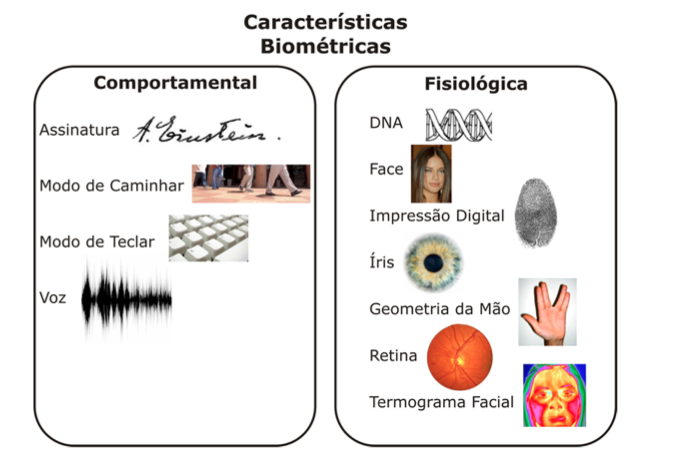
\includegraphics[height=11cm,width=17cm]{figuras/2.FundamentacaoTeorica/caracteristicasBiometricas.png}
		\end{center}
		\caption{Exemplos de algumas características biométricas \cite{drovetto}.}
		\label{caracteristicasBiometricas}
	\end{figure}

Teoricamente, qualquer característica física/comportamental pode ser utilizada para identificação caso siga alguns dos seguintes requisitos \cite{milene}: 

	\begin{enumerate}
		\item \textbf{universidade}: qualquer pessoa pode ser avaliada sobre essa característica;
		\item \textbf{singularidade}: dada duas pessoas distinas, elas não podem ter a mesma característica;
		\item \textbf{permanência}: a característica não pode mudar de acordo com o tempo;
		\item \textbf{exigibilidade}: significa que a característica pode ser mensurada quantitativamente;
	\end{enumerate}

Porém, na prática também são considerados outros requisitos \cite{milene}:

	\begin{enumerate}
		\item \textbf{desempenho}: o processo de identificação deve apresentar um resultado aceitável;
		\item \textbf{aceitação}: indica em que ponto as pessoas estão dispostas a aceitar o sistema biométrico;
		\item \textbf{evasão}: refere a facilidade de ser adulterado;
	\end{enumerate}

São várias as vatangens que os sistemas biométricos têm em relação aos sistemas convencionais. Listamos as vatagens vistas como principais \cite{drovetto}:
	
	\begin{itemize}
		\item características biométricas não podem ser perdidas ou esquecidas;
		\item características biométricas são difíceis de serem copiadas, compartilhadas e distribuídas;
		\item os sistemas biométricos necessitam que a pessoa esteja presente no local da autenticação;
	\end{itemize}

Novas técnicas de reconhecimento por meio de faces, íris, retina e voz, entre outras, têm sido abordadas para aplicações em sistemas de reconhecimento automático \cite{bolle,saocarlos}. O reconhecimento facial é apenas uma das nove características biométricas utilizadas atualmente \cite{milene}. Nas tabelas \ref{tabelaRequisitosTeoricos} e \ref{tabelaRequisitosPraticos} são mostradadas as noves características e seus respectivos comportamentos baseados nos requisitos mencionados acima.
		
	\begin{table}[htb]
		\begin{center}
			\caption{Requisitos teóricos para algoritmos de reconhecimento facial \cite{milene}.}
			\begin{tabular}{|c|c|c|c|c|}
				\hline \bf Biometria & \bf Universidade & \bf Singularidade & \bf Permanência & \bf Exigibilidade \\
				\hline \hline \bf Face & Alta & Baixa & Média & Alta \\
				\hline \bf  Digital & Média & Alta & Alta & Média \\
				\hline \bf Geometria da Mão & Média & Média & Média & Alta \\
				\hline \bf ``Hand Vein'' & Média & Média & Média & Média \\
				\hline \bf Iris & Alta & Alta & Alta & Média \\
				\hline \bf ``Retina Scan'' & Alta & Alta & Média & Baixa \\
				\hline \bf Assinatura & Baixa & Baixa & Baixa & Alta\\
				\hline \bf Voz & Média & Baixa & Baixa & Média \\
				\hline \bf Termograma & Alta & Alta & Baixa & Alta \\
				\hline
			\end{tabular}
		\end{center}
		\label{tabelaRequisitosTeoricos}
	\end{table}

	\begin{table}[htb]
		\begin{center}
			\caption{Requisitos práticos para algoritmos de reconhecimento facial \cite{milene}.}
			\begin{tabular}{|c|c|c|c|}
				\hline \bf Biometria & \bf Desempenho & \bf Aceitação & \bf Evasão \\
				\hline \hline \bf Face & Baixa & Alta & Baixa\\
				\hline \bf Digital & Alta & Média &  Alta\\
				\hline \bf Geometria da Mão & Média & Média & Média\\
				\hline \bf ``Hand Vein'' & Média & Média & Alta\\
				\hline \bf Iris  & Média & Média & Alta\\
				\hline \bf ``Retina Scan'' & Alta & Baixa & Alta\\
				\hline \bf Assinatura & Baixa & Alta & Baixa \\
				\hline \bf Voz & Baixa & Alta & Baixa \\
				\hline \bf Termograma & Média & Alta & Alta \\
				\hline
			\end{tabular}
		\end{center}
		\label{tabelaRequisitosPraticos}
	\end{table}

Um sistema biométrico responde a dois eventos: um usuário é ou não quem afirma ser. Como resposta a esses eventos, o sistema pode classificar o usuário como um cliente ou um impostor. Nessa tomada de decisão pode ocorrer dois tipos de erros: uma falsa aceitação, ao aceitar um impostor, (\textit{False Acceptance} - FA) ou uma falsa rejeição (\textit{False Rejection} - FR), ao rejeitar um cliente. Baseado nesses erros, duas taxas são utilizadas para avaliar sistemas biométricos: taxa de falsa aceitação (\textit{False Acceptance Rate} - FAR) e taxa de falsa rejeição (\textit{False Rejection Rate} - FRR) \cite{drovetto}.

A FAR é a probabilidade de um sistema biométrico aceitar um impostor como cliente. Ela é calculada pela equação (2.1) em que $\displaystyle Nfa$ é o número de falsas aceitações e $\displaystyle Ni$ é o número de impostores que tentaram acessar o sistema. A variação da taxa é representada pelo intervalo fechado $\displaystyle [0,1]$, onde o valor $\displaystyle 1$ significa que todos os impostores foram falsamente aceitos e o valor $\displaystyle 0$ significa que todos impostores foram identificados como tao. Logo quando menor o FAR mais seguro o sistema é \cite{drovetto}.

	\begin{equation}
		FAR = \frac{Nfa}{Ni} \cite{drovetto}
	\end{equation} 

A FRR é a probabilidade de um sistema biométrico rejeitar um cliente e classifica-lo como impostor. Ela é calculada pela equação (2.2) em que $\displaystyle Nfr$ é o número de falsas rejeições e $\displaystyle Nc$ é o número de clientes que tentaram acessar o sistema. A variação da taxa é representada pelo intervalo fechado $\displaystyle [0,1]$, onde o valor $\displaystyle 1$ significa que todos os clientes foram falsamente rejeitados e o valor $\displaystyle 0$ significa que todo os cliente foram aceitos corretamente. Em sistemas cuja performance tem maior grau de prioridade que a segurança, deve-se reduzir a FRR para minimizar a ocorrência de falsas rejeições \cite{drovetto}.

	\begin{equation}
		FRR = \frac{Nfr}{Nc} \cite{drovetto}
	\end{equation} 

A partir dessas taxas de erro, pode-se obter outras medidas como a \textit{Equal Error Rate} (ERR). Esta corresponde a taxa de erro na qual a tanto a FAR quanto a FRR possuem o mesmo valor. Como diferentes sistemas têm comportamentos diferentes, a ERR normalmente é utilizada para uma comparação mais rigorosa entre o sistemas. Quanto menor for a ERR, mas presciso é considerado o sistema \cite{drovetto}.

	\section{Reconhecimento Facial}

O reconhecimento facial é uma das atividades mais comuns realizadas diariamente por seres vivos dotados de certa inteligência. Essa simples atividade vem despertando o interesse de pesquisadores que trabalham com Visão Computacional e Inteligência Artificial. O objetivo desses pesquisadores é de construir sistemas artificiais capazes de realizar o reconhecimento de faces humanas e a partir desta capacidade construir os mais diferentes tipos de aplicações: sistemas de vigilância, controles de acesso, definções automáticas de perfis, entre outros \cite{oliveira}.

No anos 70, os estudos do reconhecimento facial eram baseados sobre atributos faciais mensuráveis como olhos, nariz, sobrancelhas, bocas, entre outros. Porém, os recursos computacionais eram escassos e os algoritmos de extração de características eram ineficiêntes. Nos anos 90, as pesquisas na área ressurgiram, inovando os métodos existentes \cite{hong, saocarlos} e disseminando a técnica.

Um dos motivos que incentivou os diversos estudos sobre reconhecimento facial são as vantagens que o mesmo possui em relação a impressão digital e a íris.  No reconhecimento por impressão digital, a desvantagem consiste no fato que nem todas as pessoas possuem uma impressão digital com ``qualidade'' suficiente para ser reconhecida por um sistema. Já o reconhecimento por íris apresenta uma alta confiabilidade e larga variação, sendo estável pela vida toda. Porém, a desvantagem está relacionada ao modo de captura da íris que necessita de um alinhamento entre a câmera e os olhos da pessoa \cite{saocarlos}. 

Basicamente existem duas particularidades que fazem da face uma característica biométrica bastante atrativa \cite{drovetto}:

	\begin{enumerate}
		\item A aquisição da face é feita de forma fácil e não-intrusiva;
		\item Possui uma baixa privacidade de informação: como a face é exposta constantemente, caso uma base de faces seja roubada, essas informações não representam algum risco e não possibilitam um uso impróprio;
	\end{enumerate}

Umas das maiores dificuldades dos sistemas de reconhecimento é tratar a complexidade dos padrões visuais. Mesmo sabendo que todas as faces possuem padrões reconhecidos, como boca, olhos e nariz, elas também possuem variações únicas que devem ser utilizadas para determinar as características relevantes. Outra dificuldade encontrada em relação a essas características é que elas possuem uma larga variação estatística para serem consideradas únicas para cada indivíduo. O ideal seria que a variância inter-classe seja grande e a intra-classe pequena, pois assim imagens de diferentes faces geram os códigos mais diferentes possíveis, enquanto imagens de uma mesma face geram os códigos mais similares possíveis. Portanto, estabelecer uma representação que capture as características ideias é um difícil problema \cite{saocarlos}.

Do ponto de vista geral, o recohecimento facial continua sendo um problema aberto por causa de várias dificuldades que aumentam a variância intra-classe \cite{hong}. Entre estas, destacamos as mais comuns \cite{saocarlos}:

	\begin{itemize}
		\item iluminação;
		\item ângulos e poses;
		\item expressões;
		\item comésticos e acessórios;
		\item extração da face do contexto ou do fundo;
	\end{itemize}

No contexto de identificação, o reconhecimento facial se resume no reconhecimento de um ``retrato'' frontal, estático e controlado. Estático pois os ``retratos'' utilizados nada mais são que imagens, podendo ser tanto de intensidade quanto de profunidade e controlado pois a iluminação, o fundo, a resolução dos dispositivos de aquisição e a distância entre eles e as faces são essencialmente fixas durante o processo de aquisição da imagem \cite{hong}.

Basicamente, o processo de reconhecimento facial pode ser divido em duas tarefas principais \cite{hong}:

	\begin{enumerate}
		\item Detecção de faces em imagens;
		\item Reconhecimento das faces encontradas;
	\end{enumerate}

Falaremos dessas duas tarefas separadamente nas próximas subseções.



\subsection{Detecção de Faces em imagens}
	
A primeira etapa para o reconhecimento de faces é a detecção de um rosto, e a partir daí a comparação do mesmo com modelos conhecidos pelo sistema \cite{hong, oliveira}. Em um sistema de reconhecimento facial, tanto o tempo de resposta quanto a confiabilidade desta etapa influência diretamente no desempenho e o emprego deste sistema \cite{oliveira}.

A detecção de faces é definida como o processo que determina a existência ou não de faces em uma imagem e uma vez encotrada alguma face, sua localização deve ser apontada através de um enquadramento ou através de suas coordenadas dentro da imagem \cite{oliveira}. A figura \ref{enquadramentoRosto} representa um exemplo da detecção de uma face em uma imagem.

	\begin{figure}[hbt]
		\begin{center}
			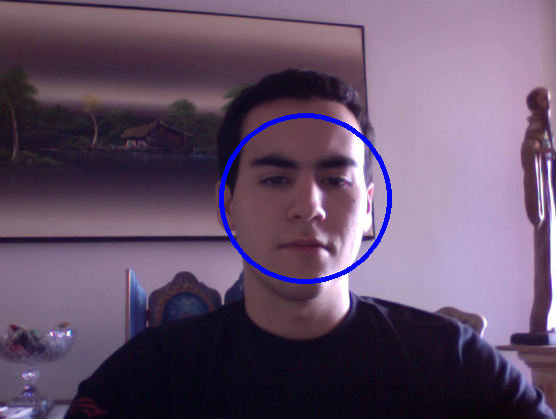
\includegraphics[height=9.5cm,width=12.5cm]{figuras/2.FundamentacaoTeorica/enquadramentoRosto.png}
		\end{center}
		\caption{Exemplo de um processo de detecção de uma face em uma imagem.}
		\label{enquadramentoRosto}
	\end{figure}

O processo de detecção de faces geralmente é pelas seguintes razões mostradas a seguir:

	\begin{enumerate}
		\item \textbf{Pose}: as imagens de uma face podem variar de acordo com a posição relativa entre a camêra e a face (frontal, 45 graus, perfil, ``de cabeça para baixo''), e com isso algumas características da face, como olhos e nariz, podem ficar parcialmente ou totalmente ocultadas \cite{yang}.
		\item \textbf{Presença de acessórios}: características faciais básicas importantes para o processo de detecção podem ficar ocultadas pela presença de acessórios, como óculos, bigode, barba, entre outros \cite{oliveira, yang}. 
		\item \textbf{Expressões faciais}: embora a maioria das faces apresente estruturas semelhantes (olhos, bocas, nariz, entre outros) e são dispostas aproximadamente na mesma configuração de espaço, pode haver um grande número de componentes não rigídos e texturas diferentes entre as faces. Um exemplo são as flexibilizações causadas pelas expressões faciais \cite{oliveira, yang};
		\item \textbf{Obstrução}: faces podem ser obstruídas por outros objetos. Em uma imagem com várias faces, uma face pode obstruir outra \cite{yang}.
		\item \textbf{Condiçoes da imagem}: a não previsibilidade das condições da imagem em ambientes sem restrições de ilimuniação, cores e objetos de fundo \cite{oliveira, yang}.
	\end{enumerate}

Atualmente, já existem diferentes métodos/técnicas de detecção de faces. Faleremos um pouco sobre os métodos baseados em imagens de itensidade e de cor e depois falaremos sobre os baseados em imagens 3D.

Um problema relacionado e muito importante é como avaliar a performance dos métodos de detecção de faces propostos. Com isso, muitas métricas foram adotadas como tempo de aprendizagem, número de amostras necessárias no treinamento e a proporção entre taxas de detecção e ``falso alarme''. Esta última é dificultada pelas diferentes definições para as taxas de detecção e falso alarme adotadas pelos pesquisadores \cite{yang}.

% ##################################################################################################################
% ##################################################################################################################
% ##################################################################################################################

\subsection{Reconhecimento das Faces encontradas}

Na etapa de reconhecimento, as faces detectadas e processadas, serão comparadas com um banco de dados de faces conhecidas. Essa comparação tem uma acurácia media de 30-90\% entre as diversas técnicas []. Esse é um forte campo de pesquisa desde a década de 90 e as técnicas se invovam ano ápos ano.

	Técnicas 2D:
	\begin{enumerate}
		\item \textbf{Eigenfaces} []
		\item \textbf{Redes Neurais} []
		\item \textbf{Fisher Faces} []
	\end{enumerate}

Com o surgimento da tecnologia 3D o reconhecimento facial se trasformou mais confiável pois a imagem 3D evita problemas comum em reconhecimentos faciais 2D como a mudança na iluminação, diferentes expressões faciais, maquiagem e orientação da cabeça.
	Técnicas 3D:
	\begin{enumerate}
		\item \textbf{``Face Recognition Homepage''} []
		\item \textbf{``3D Face Recognition''} []
		\item \textbf{``Active Appearance Models''} []
	\end{enumerate}


O Eigenface é um algoritmo de reconhecimento facial 2D simples e fácil de implementar. Os passos utilizados pelo Eigenface também são utilizados em muitos métodos avançados. Os princípios básicos por trás dele como PCA(``Principal Component Analisys'') e ``distance-based matching'' aparecem mais e mais na computação visual e aplicações diversas de maquinas inteligentes.
O Eigenface trabalha de forma simples, dada uma imagem de um rosto desconhecido e imagens do rosto das pessoas conhecidas executa as seguintes ações.
	\begin{enumerate}
		\item Computa a distância entre a nova imagem e cada uma das imagens já conhecidas.
		\item Seleciona a imagem mais proxima do novo rosto.
		\item Se a distância da nova imagem para a imagem exemplo for maior que o limite predefinido, ``reconhece'' a imagem caso contrario classifica como ``desconhecida''.
	\end{enumerate}


A distância entre as imagens é medida ponto a ponto. Esta é também chamado de distância euclidiana. Em duas dimensões (2D), a distância euclidiana entre os pontos $P_1$ e $P_2$ é dada pela fórmula $\displaystyle d_{12} = \sqrt(d_{x2} + d_{y2})$, onde $\displaystyle d_x = x_2 - x_1$ e $\displaystyle d_y = y_2-y_1$ e representada na Figura \ref{distanciaEntrePontos}.

    \begin{figure}[hbt]
		\begin{center}
			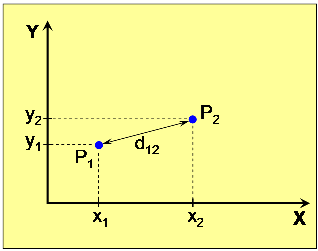
\includegraphics[height=9.5cm,width=12.5cm]{figuras/2.FundamentacaoTeorica/graficoDistanciaEntrePontos.png}
		\end{center}
		\caption{Distância Euclidiana entre dois pontos em duas dimensões.}
		\label{distanciaEntrePontos}
	\end{figure}


Imagens possuem ``ruídos'' e vamos definir ruído como qualquer coisa que atrapalhe na identificação, como por exemplo as diferenças na luminosidade. Cada pixel possui uma intensidade de ruído diferente e com cada pixel dando a sua contribuição fica muito difícil encontrar a imagem correta. Uma solução é diminuir a dimensionalidade da imagem tornando assim o ruido menor e sendo possível extrair as informações importante da imagem.

Um dos métodos existentes para redução de imagem é o ``PCA - Principal Components Analysis''.

Para se ter uma idéia do que é o PCA, vejamos um caso especial chamado de ``least squares line fit''. O lado esquerdo da Figura \ref{exemploPCA} mostra um exemplo de uma linha média entre três pontos, que são, no mapa em 2D, Los Angeles, Chicago e Nova York. Estes três pontos do mapa são quase, mas não completamente, uma única linha. Se você estava planejando uma viagem, essa relação já seria uma informação útil. Nesse sentido, uma única linha expressa algo essencial sobre seu relacionamento. A linha tem apenas uma dimensão, por isso, se podemos substituir localizações dos pontos de 2D com localizações ao longo de uma única linha, vamos ter reduzido a sua dimensionalidade.

Como eles já estão quase alinhados, uma linha pode ser traçada através deles com pouco erro. O erro no ajuste da linha é medido pela soma do quadrado da distância de cada ponto da linha. A linha de melhor ajuste é aquela que possui o menor erro.

	\begin{figure}[hbt]
		\begin{center}
			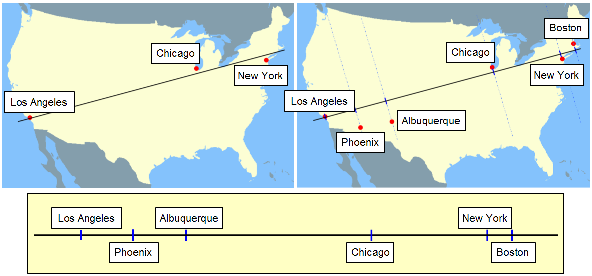
\includegraphics[height=9.5cm,width=12.5cm]{figuras/2.FundamentacaoTeorica/PCAexemploMapa.png}
		\end{center}
		\caption{Mapa exemplo para redução de dimensionalidade}
		\label{exemploPCA}
	\end{figure}

Embora a linha encontrada acima é um objeto 1D, é localizado dentro de um espaço maior, 2D, e tem uma orientação, sua inclinação. A inclinação da linha expressa algo importante sobre os três pontos. Ele indica a direção em que eles estão mais espalhados.


Se posicionarmos a origem do nosso plano cartesiano em algum lugar dessa linha, podemos escrever a equação da linha como uma simples $y = mx$, onde m é a inclinação da linha: $dy / dx$.

Quando ele é descrito desta maneira, a linha é um subespaço do espaço 2D definido pelo sistema de coordenadas. Esta descrição enfatiza o aspecto dos dados que estamos interessados, ou seja, a direção que mantém esses pontos mais separados um do outro.

Esta direção da separação máxima é chamada de primeira componente principal de um conjunto de dados. A próxima direção com máxima separação é a perpendicular a esta. Essa é a segunda componente principal. Em um conjunto de dados 2D, podemos ter no máximo duas componentes principais.

No entanto, o número de componentes principais que podemos encontrar também é limitada pelo número de pontos de dados. Para ver o porque disto, podemos pensar em um conjunto de dados que consiste de apenas um ponto. Não há sentido da separação máxima para esse conjunto de dados, porque não há nada para separar. Agora, considere um conjunto de dados com apenas dois pontos. A linha que conecta esses dois pontos é a primeira componente principal. Mas não há uma segunda componente principal, porque não há nada mais para separar, pois os dois pontos estão totalmente na linha.

Em Eigenface, cada imagem da face, de tamanho 50x50, é tratada como um ponto (com espaço dimensional de 2500). Portanto, o número de componentes principais, podemos encontrar nunca será mais do que o número de imagens de faces menos um.

Embora seja importante ter um entendimento conceitual do que as componentes principais são, você não precisa saber os detalhes de como encontrá-las para implementar o Eigenface. Essa parte já foi implementada em bibliotecas de processamento de imagens \textit{open source}, como por exemplo a bliblioteca ``OpenCV''.

Voltando ao mapa da Figura \ref{exemploPCA}, agora que nós encontramos um subespaço 1D, temos uma maneira de converter os pontos em 2D para 1D. Esse processo se chama projeção. Para projetar um ponto do mapa para a linha, você encontra o ponto da linha que está mais próximo do ponto 2D. Essa é sua projeção.

Há uma função no ``OpenCV'' para projetar os pontos sobre um subespaço, então, novamente, você só precisa de um entendimento conceitual. Você pode deixar os detalhes algorítmicos para a biblioteca.

As marcas azuis na Figura \ref{exemploPCA} mostram as localizações no subespaço das três cidades que definiram a linha. Outros pontos 2D também pode ser projetado para esta linha. O lado direito da Figura \ref{exemploPCA} mostra a localização prevista para Phoenix, Albuquerque, Boston.

Em Eigenface, a distância entre duas imagens é a distância euclidiana entre os pontos projetados em um subespaço, ao invés da distância no espaço original da imagem de 2500 dimenções. A distância entre as faces neste subespaço de menor dimensão é a técnica utilizada para melhorar a relação sinal / ruído.

Muitas técnicas avançadas de reconhecimento de face são extensões deste conceito básico. A principal diferença entre Eigenface e estas técnicas avançadas é o processo de definição do subespaço. Em vez de usar PCA, o subespaço pode ser baseada em Análise de Componentes Independentes (ICA) ou em Análise Discriminante Linear (LDA), e assim por diante.

Em nossa definição de uma linha como um subespaço 1D, usamos X e Y coordenadas para definir m, que é sua inclinação em 2D. Quando m é um componente principal de um conjunto de pontos, ela é chamada de autovetor ou ``eingenvector'', daí o nome eigenface. 

Para o reconhecimento facial em imagens de 50x50, cada autovetor representa a inclinação de uma linha em um espaço de 2.500 dimenções. Como no caso 2D, precisamos de todas as 2.500 dimensões para definir a inclinação de cada linha. Embora seja impossível visualizar uma linha em muitas dimensões, podemos visualizar os autovetores de uma maneira diferente. Podemos converter as suas 2.500 dimenções em uma simples imagem usando a sua ``inclinação'' para colocar cada pixel valor em seu local correspondente. Quando fazemos isso, obtemos imagens ``facelike'' chamadas de eigenfaces.

Eigenfaces é um método interessante para dar-nos alguma intuição sobre os componentes principais para o nosso conjunto de dados. O lado esquerdo da Figura \ref{exemploEigenfaces} mostra as imagens das faces de dez pessoas. Estas imagens foram encontradas no ``Yale Face Database B (referências 4 e 5)''. Ele contém imagens de rostos com uma variedade de condições de iluminação. Foram usadas sete imagens de cada uma dessas dez pessoas para criar um subespaço PCA. 

O lado direito da Figura \ref{exemploEigenfaces} mostra os seis primeiros componentes principais deste conjunto de dados, apresentados como eigenfaces. O eigenfaces muitas vezes têm um olhar fantasmagórico, porque combinam elementos de várias faces. As regiões de pixels mais brilhantes e as regiões mais escuras em cada imagem foram os que mais contribuíram para esse componente principal. 

	\begin{figure}[hbt]
		\begin{center}
			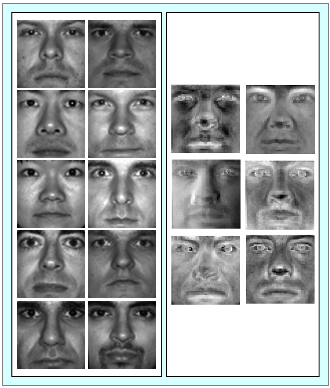
\includegraphics[width=12cm]{figuras/2.FundamentacaoTeorica/eigenfaces.png}
		\end{center}
		\caption{Direita: imagens de rosto para dez pessoas. Esquerda: os seis primeiros componentes principais, visto como eigenfaces.}
		\label{exemploEigenfaces}
	\end{figure}

Os principais componentes que encontra APC são os rumos da maior variação nos dados. Um dos pressupostos na Eigenface é que a variabilidade nas imagens subjacente corresponde à diferença entre as faces individuais. Esta suposição é, infelizmente, nem sempre válido. A Figura \ref{exemplosImagensIluminacaoo} mostra os rostos de duas pessoas. A face de cada indivíduo é apresentada em quatro diferentes condições de iluminação.

Estas imagens são também do ``Yale Face Database B''. Na verdade, eles são imagens de faces de duas das dez pessoas mostrado na Figura \ref{exemploEigenfaces}. Você pode dizer qual é qual? Eigenface não pode. Quando a iluminação é muito variável, Eigenface muitas vezes não o faz melhor palpite aleatório faria.

	\begin{figure}[hbt]
		\begin{center}
			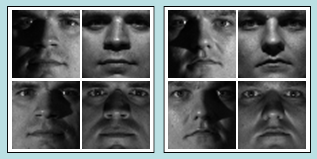
\includegraphics[width=14cm]{figuras/2.FundamentacaoTeorica/exemplosImagensIluminacaoo.png}
		\end{center}
		\caption{Face imagens de dois indivíduos. A face de cada indivíduo é apresentada em quatro diferentes condições de iluminação. A variabilidade devido à iluminação aqui é maior do que a variabilidade entre os indivíduos. Eigenface tende a confundir as pessoas quando os efeitos de iluminação são fortes.}
		\label{exemplosImagensIluminacaoo}
	\end{figure}


%Como mencionado em cima, essa idéia básica - redução de dimensionalidade seguido pelo cálculo da distância em um subespaço - é amplamente utilizado no trabalho de visão computacional. Também é utilizado em outros ramos da AI. Na verdade, é uma das principais ferramentas para gerenciar a complexidade e para encontrar padrões escondidos dentro de enormes quantidades de dados do mundo real.




% Os métodos baseados em imagens de intensidade e cor podem ser divididos em 4 categorias \cite{yang}:

% 	\begin{enumerate}
% 		\item \textbf{``Knowladge-based methods'':} métodos, desenvolvidos principalmente para localização facial, beaseados em regras derivadas do conhecimento dos pesquisadores do que constitui uma típica face humana. Normalmente, captura as relações existentes entre as características faciais. É fácil econtrar regras que descrevem as caracterísicas faciais. Por exemplo, uma face sempre é constituída por dois olhos simétricos, um nariz e uma boca. As relações entre essas características podem ser representadas pelas distâncias relativas e posições.  \cite{yang};

% 		\item \textbf{``Feature invariant approaches'':} esses algoritmos tem como objetivo principal encontrar as características estruturais que existem mesmo quando a postura, ``ponto de vista'', condições de iluminação variam. E por meio dessas características localizar a face. São desenvolvidos principalmente para localização facial \cite{yang};

% 		\item \textbf{``Template matching methods'':} vários padrões comuns de um rosto são armazenados tanto para descrever o rosto como um todo quanto para descrever as características faciais separadamente. As correlações entre as imagens de entrada e os padrões armazenados são comuptados para detecção. Esses métodos são desenvolvidos para serem utlizados como localização e detecção facial \cite{yang};

% 		\item \textbf{``Appearence-based methods'':} Em contraste com os métodos do item anterior, os modelos são retirados de um conjunto de imagens de treinamento que devem capturar a variabilidade da face. Esses modelos retirados são utilizados para detecção. São métodos desenvolvidos principalmente para detecção de faces \cite{yang};

% 	\end{enumerate}





























